% !TEX root = SocialVision2012.tex

\subsection{Datasets and Challenge Problems}
\label{sec:sys}

\begin{figure}[t!]
\begin{center}
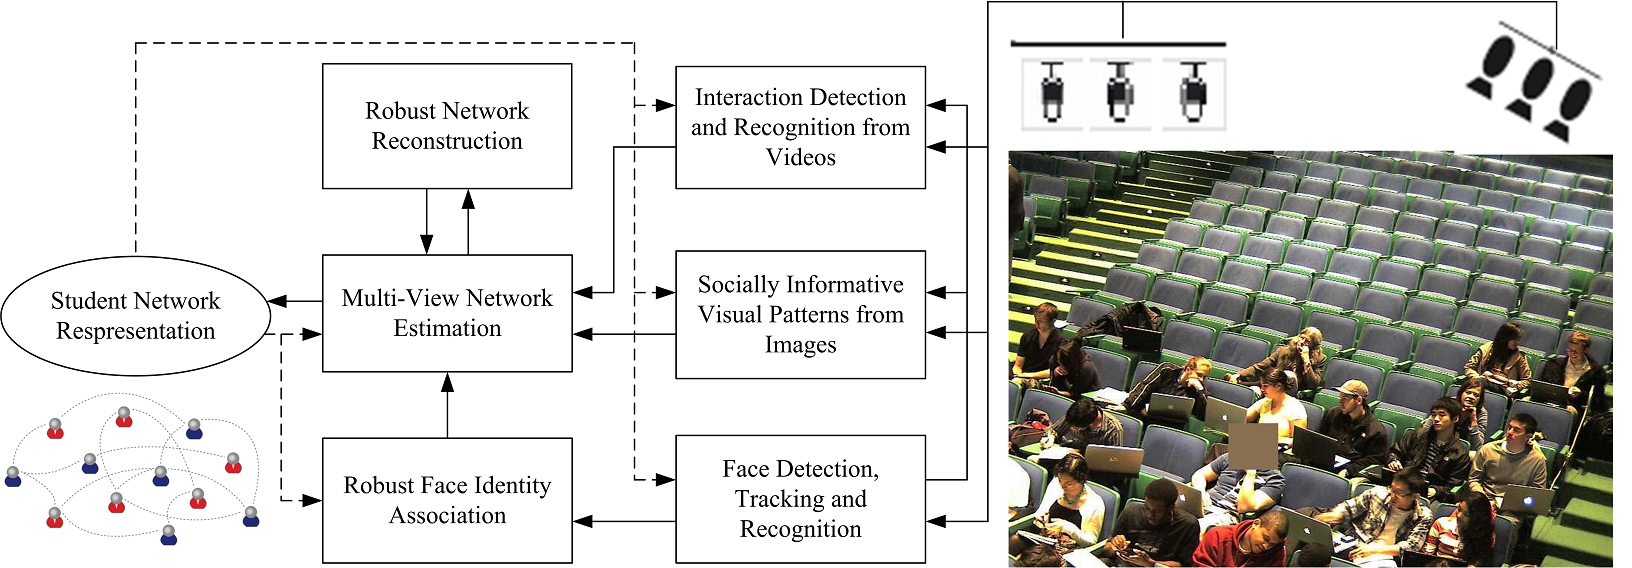
\includegraphics[width=\columnwidth]{prototype_1}
\end{center}
\vspace{-0.25in} \caption{\captionsize 
(a) The prototype hardware and software infrastructure for analyzing moderately constrained socialized human behaviors in an indoor environment for social network estimation at Harvard University; (b) Severely constrained UT Interaction dataset \cite{UTdata}; (c) Unconstrained New York Grand Central Station dataset \cite{WangMG09}.}\label{fig:prototype}\end{figure}

Our goal is to build a foundation for social analysis in diverse, unconstrained environments like that depicted in the bottom-right of Fig.~\ref{fig:prototype}(a). This is becoming well within reach thanks to the ready availability of networked camera arrays and advances in practical multi-view detection and tracking (e.g.,~\cite{EshelM10}). These unconstrained environments are fundamentally different from scenarios considered in existing benchmark datasets for interaction analysis (Fig.~\ref{fig:prototype}(b)(c)), where the interactions involve a pre-determined number of participants; take place in the absence of by-standers or social clutter; and/or are localized in time \emph{a priori}~\cite{UTdata,Choi:context,Choi:recogtrack,CRIM13}. Because of these  differences, evaluations on existing benchmarks fail to provide meaningful proxies for fundamental progress in large-scale social visual analysis.

As part of the proposed activity, we will create new datasets and challenge problems that make it possible to measure meaningful progress on social visual analysis, and at the same time, serve as a mechanism to engage the broader computer vision research community. To ensure that our benchmarks provide effective measures of progress, they will be annotated with ground-truth information about identities, interaction categories, and social relationships. We will create and use two distinct types of datasets. The first type will be based on video collections that are already being collected in large interactive classrooms at Harvard University. These datasets will be large (more than \todd{350} camera-hours of video have been collected so far) and will enable evaluation of all aspects of the proposed research program, but because of the need for maintaining privacy of the observed subjects they will not be made directly available to non-collaborating research groups. The second type of datasets will supplement the first by being made publicly available. These will be smaller collections of annotated videos that contain interactions staged by informed actors, and they will simulate unconstrained environments by including long videos of large social gatherings. These will enable the evaluation of some aspects of the proposed research program (e.g., detecting interaction categories) and will be presented as ``challenge problems" for the broader computer vision research community.

\subsubsection{Harvard Interactive Classroom Datasets}
We will leverage video that is currently being collected by a six-camera array in a large interactive classroom at Harvard University. This system, which we call ``Lens to Learning'', has been developed over the past three years with funding by the NSF (IIS-0835338, 2009--2012) and the Harvard Initiative for Learning and Teaching (HILT)\footnote{\href{http://hilt.harvard.edu/2012-2013-awards}{http://hilt.harvard.edu/2012-2013-awards}} with the goal of understanding how students learn in interactive classrooms. The observed classroom is ``interactive'' in that students frequently engage in ad-hoc discussions. One commonly used technique is \emph{Peer Instruction}, which involves brief student discussions during the time traditionally devoted to lecture. Each discussion begins with a single ConcepTest---a question designed to elicit common student misconceptions [19,70]. The students are given a moment to formulate and electronically submit their individual answer to the question posed, and then they are asked to form ad-hoc discussion groups to try to convince neighboring students of the correctness of their answers. After a few minutes of peer-to-peer discussion, students submit their possibly-revised answers, and this entire activity is usually followed by the instructor�s reinforcement of the main concept. Education research shows that both high and low ability students benefit from these discussions [24,36,80,83].

The videos collected by Lens to Learning present an extraordinary opportunity for developing and evaluating large-scale social visual analysis. The observed classrooms---part of one is shown in Fig.~\ref{fig:prototype}(a), contain a hundred or more individuals engaged in ad-hoc interactions, and this creates a social environment that is fundamentally different from previous datasets (e.g., Fig.~\ref{fig:prototype}(b)(c)) in which interactions are  pre-localized in space or time. The utility of our interactive classrooms for social visual research stems not only from the number and diversity of people they contain, but from the nature of the interactions, the duration of our observations, and the non-visual sources of metadata available for validation. Individuals typically remain seated and forward-facing, and this simplifies detection and tracking, allowing us to focus our research on the higher-level challenges of detecting and recognizing social interactions. Also, for each course, videos are collected in every lecture over three-month semesters (about 200 camera-hours per course), enabling thorough evaluation of our methods for aggregating visual interaction data to infer social network information. This evaluation is made meaningful because of immense efforts being made by educational experts (funded by other sources and using techniques like those in [92]) to define a small number of semantically-meaningful interaction categories and painstakingly annotate occurrences of these interactions in the videos. This means, for example, that we can use the proposed techniques to discover and detect large numbers of interaction categories and then measure the degree to which some of them agree with the much smaller number that could be analyzed by human experts. Furthermore, in addition to video data, we have access to many non-visual sources of social network information (audio recordings from 48 omnidirectional boundary microphones mounted inconspicuously among the seats; educational outcomes; answers to ConcepTests; section assignments; gender; age; ethnicity; housing assignments, etc.) that allow some cross-validation of the social networks that we reconstruct from visual data.

To automatically analyze the videos collected by the Lens to Learning system, we have already developed a  suite of computer vision tools for ``pre-processing'' via face and body detection and tracking. This includes implementations of face detection and tracking, identity recognition, and head pose estimation, that together  provide large numbers of time-varying individual and pairwise descriptors ($\mathbf{f}_{m,t}$ and $\mathbf{g}_{m,m',t}$ in Section~\ref{sec:activity}) to be used as input to our methods. This dataset is affected by many sources of noise (false detections, missed detections, uncertain identities, uncertain pose) and is therefore a good proxy for many real-world environments. While this pre-processing suite provides a useful starting point for our research, we will continue to develop it during the award period to include richer descriptors such as histograms of flow and space-time interest points that capture elements of body pose and gesture. 

In conjunction with the Institutional Review Board at Harvard University, we have established a protocol in which classroom videos are recorded with consent from students and instructors, and then stored and analyzed on VPN-protected servers. More than 95\% of students also provide consent for their videos to appear in academic publications and presentations, allowing us to disseminate our research results through all of the regular academic channels. But since the classroom videos cannot be made directly available to research groups other than ours, we will promote reproducible research in three different ways. First, as described in the next section, we will create smaller parallel  datasets that are publicly-available and allow other research groups to evaluate algorithms for certain aspects of social visual analysis. Second, we will welcome interested research groups to collaborate with us to evaluate their algorithms on our classroom data by running their code on our VPN-protected servers. Third, whenever possible we will make use of advancing  technologies for privacy-preserving social science research---like those currently being developed by colleagues at Harvard University\footnote{\href{http://privacytools.seas.harvard.edu}{http://privacytools.seas.harvard.edu}}---to enable more direct sharing of classroom data for research purposes.

\subsubsection{Challenge problems}

An encouraging trend in computer vision over the last several years has been the increasing use of benchmark datasets for evaluating progress on particular tasks. Standardized datasets, such as the Middlebury Stereo Evaluation project~\cite{ScharsteinS02}, the PASCAL VOC Challenges~\cite{Everingham10}, the Berkeley Segmentation Database~\cite{MartinFTM01}, and the KTH database of individual actions~\cite{KTH}, have served as catalysts for progress on difficult problems because they create concrete targets that inspire new ideas and allow researchers to evaluate their systems by quantitatively demonstrating improvement. Currently, there are relatively few datasets available for problems related to social visual analysis, and those that do exist consider severely constrained environments that are not good proxies for the real world.

As part of the proposed activity, we will create new datasets and define challenge problems that engage the computer vision research community in our research agenda. \todd{Need more here -- details about a staged interaction dataset that we will create to evaluate interaction detection}

We will publish side-by-side comparisons of our performance on these public shared benchmarks and corresponding benchmarks derived from our  private classroom data. This is a strategy that PI Zickler has previously employed for research on private photo collections~\cite{PintoZickler2011}, and it means that any researcher who evaluates their algorithms on our (staged) public datasets can obtain an estimate of how well those same algorithms would perform in a  real classroom environment.


%With this established classroom observation system and these fundamental modules, we have successfully collected and processed a large-scale classroom behavior database consisting of 100 video clips in total. The students are seated in a regular lecture hall and are observed by a camera array with non-overlapping fields of view. The classroom is ``interactive'' because at various times throughout the lecture students are invited to engage in ad-hoc group discussions about problems provided by the instructor. The scale of our database is orders of magnitude larger than state-of-the-art computer vision datasets (e.g. those used in \cite{UTdata,Choi:context,Choi:recogtrack}), in the number of individuals (10-50 students per camera), the number of cameras (6), and the amount of time (100 minutes per camera, per recording, equaling over 3,000 minutes in total). Through a combination of face detection and tracking, we obtained noisy tracks for all students in each monocular video, upon which we developed descriptive modules that directly extract descriptiors such as head pose and body motion, we have also implemented a high-level module for behavior analysis based on similarity between two social groups, as depicted in Fig. \ref{fig:prototype}(b). In this module, the behavior of each individual is represented by a combination of the head pose and the motion of torso and arms (using the method of histogram of optical flows). The social behavior of a group is then represented by the configuration in space and time of the behaviors of its participants. With this social activity representation, the module detects a salient social activity from a new video and retrieves similar social activities from our established database. This functionality is illustrated in Fig. \ref{fig:prototype}(b), where our system has discovered a three-way conversation by identifying the participants of this conversation and the time span (several to tens of seconds) of this event. Based on the behavior representation for this space-time social interaction, the system searches the remainder of the database and retrieves a list of exemplars containing similar social behavior, ranked in the descending order of the similarities with the query. In this way, any manual annotations associated with the query video can be propagated to the top-ranking exemplars, and we are now taking this approach to propagate our manual annotations across the whole database. 








%At the current and initial stage of the effort to bring socialized semantics to computer vision, it can be usually the case that we do not have sufficient social contexts to help improving our target/face recognition, and we are not always specific about what are the meaningful social interactive activities that are most informative for social description. Conversely, we may neither know clearly about what exactly we should distill from images to fulfill a network learning task, nor have concrete knowledge about how the multiple views or overlapping community structures of a network will eventually turn out to be. However, we have argued at the beginning and demonstrated through the four proposed research problems the fact that the two aspects assist and benefit from each other, and an overall socially-aware visual analytical system is our ultimate goal. To this end, our final proposed research will include an attempt for a framework that eventually integrate social information and image understanding and allow them to learn and self-build themselves in an evolving and unsupervised manner.





